\newcommand{\reporttitle}{CMOS Τελεστικός Ενισχυτής Δύο Σταδίων}
\newcommand{\authorOne}{Καπετάνιος Αντώνιος}
\newcommand{\aemOne}{10417}

\documentclass[10pt,a4paper]{article}
\usepackage[fontsize=9pt]{scrextend}
\usepackage[portrait,textwidth=18cm,top=1cm,bottom=2cm,includeheadfoot]{geometry}
\usepackage{amsmath,amsfonts,amssymb,mathtools,xfrac,siunitx,stmaryrd}
\usepackage{enumitem}
\usepackage{fancyhdr}
\usepackage{float,newfloat}
\usepackage{graphicx}
\usepackage{dcolumn,tabularx,longtable,multirow,subfigure,caption}
\def\greekOptions{chapterhead=unchanged}
\usepackage[english,main=greek]{babel}
\usepackage{amsmath,amsfonts,amssymb,mathtools,xfrac,halloweenmath}
\usepackage[LGR]{fontenc}
\usepackage{fontspec}
\usepackage[normalize-symbols]{textalpha}
\usepackage{unicode-math}
\setmathfont{Concrete-Math.otf}
\setmainfont{GFS Neohellenic}
\usepackage{indentfirst}
\usepackage[x11names]{xcolor}
\usepackage[unicode,luatex,hidelinks]{hyperref}
\hypersetup{pdftitle={Microelectronics III},
			pdfsubject={Two-stage MOSFET operational amplifier},
			pdfauthor={\authorOne~[\aemOne]},
			bookmarksnumbered=true,
			bookmarksopen=true}
\usepackage[all]{hypcap}
\usepackage{tikz}
\usetikzlibrary{matrix,backgrounds}
\usepackage{steinmetz}
\usepackage{titlesec}
\usepackage{etoolbox}
\usepackage{pgfplots}
\usepackage{wrapfig}
\usepackage[language=greek,bibencoding=utf8,backend=biber]{biblatex}
\addbibresource{references.bib}
\usepackage{multicol}
\usepackage[titletoc]{appendix}
\usepackage{matlab-prettifier}

\pdfvariable minorversion=5
\pdfvariable compresslevel=9

% =====================================================================================================

\let\oldcite\cite
\renewcommand{\cite}[1]{\textcolor{darkgray}{\textsuperscript{\footnotesize\oldcite{#1}}}}
\newfontfamily\chfnt{GFS Didot}
\DeclareFloatingEnvironment[name={Κύκλωμα}]{circuitfig}
\DeclareFloatingEnvironment[name={Διάγραμμα}]{plotenv}
\newcommand{\dd}[1]{\,\mathrm{d}{#1}}
\newcommand{\GB}{\mathrm{GB}}
\newcommand{\SR}{\mathrm{SR}}
\renewcommand{\(}{\left(}
\renewcommand{\)}{\right)}
\newcommand{\lb}{\llbracket}
\newcommand{\rb}{\rrbracket}
\newcommand{\kohm}{\unit{\kilo\ohm}}
\newcolumntype{d}[1]{D{.}{.}{#1}}
\setlength{\headheight}{14.5pt}
\renewcommand{\headrulewidth}{0.1pt}
\renewcommand{\footrulewidth}{0.1pt}
\captionsetup{font=small,labelfont=bf}\numberwithin{equation}{section}
\numberwithin{equation}{subsection}

\patchcmd\subequations
 {\theparentequation\alph{equation}}
 {\subequationsformat}
 {}{}

\newcommand{\subequationsformat}{\theparentequation.\roman{equation}}

%--- chapter, sections...

\renewcommand{\thesection}{${\text{\chfnt\Roman{section}}}$}
\renewcommand{\thesubsection}{${\text{\chfnt\Roman{section}}}$.\arabic{subsection}}

\titleformat{\section}
	{\vspace*{0.7em}\color{DodgerBlue3}\normalfont\chfnt\Large\bfseries}{\thesection$\;$}{0.5em}{}

\titleformat{\subsection}
	{\color{DodgerBlue4}\normalfont\chfnt\large\bfseries}{\thesubsection}{0.5em}{}

%--- chapter heading

\fancypagestyle{fancy}{
	\fancyhf{}
	\fancyfoot[LE,RO]{\thepage}
	\fancyfoot[RE,LO]{\reporttitle}
    \renewcommand{\footrule}{\hbox to \headwidth{\color{gray}\leaders\hrule height \footrulewidth\hfill}}
	\renewcommand{\footrulewidth}{0.2pt}
}

\fancypagestyle{plain}{
	\fancyhf{}
	\fancyfoot[LE,RO]{\thepage}
    \renewcommand{\footrule}{\hbox to \headwidth{\color{gray}\leaders\hrule height \footrulewidth\hfill}}
	\renewcommand{\footrulewidth}{0.2pt}
}
\renewcommand{\headrulewidth}{0pt}
\pagestyle{fancy}

\addto\captionsgreek{\renewcommand{\chaptername}{Άσκηση}}

\renewcommand{\arraystretch}{1.4}

\begin{document}
	\pagenumbering{arabic}
	\begin{center}
	\noindent\textsc{{Αριστοτέλειο Πανεπιστήμιο Θεσσαλονίκης}}\\
	\noindent\textsc{{Πολυτεχνική Σχολή}}\\
	\noindent\textsc{{Τμήμα Ηλεκτρολόγων Μηχανικών	\& Μηχανικών Υπολογιστών}}\\[10pt]
	\noindent{\Large{\textbf{MOSFET Τελεστικός Ενισχυτής Δύο Σταδίων}}}\\
	\noindent\textsc{{47 --- Ηλεκτρονική ΙΙΙ}}\\[8pt]
	\noindent\small{\authorOne~[AEM \aemOne]}\\
	\noindent{\footnotesize{\texttt{kapetaat@ece.auth.gr}}}\\[8pt]
\end{center}
	\begin{abstract}
	Στην παρούσα εργασία μελετάται, σχεδιάζεται και προσομοιώνεται ένας τελεστικός ενισχυτής δύο σταδίων με διαφορικό ζεύγος διαύλου p σε τεχνολογία MOS 0.35. Όλα τα transistor είναι enhancement-mode εξαρτήματα. Δηλαδή, ο δίαυλος δεν είναι προκατασκευασμένος, αλλά δημιουργείται με την εφαρμογή δυναμικού στον gate ακροδέκτη του transistor.\cite{jaeger} Επιπλέον, ο ακροδέκτης του substrate τους είναι βραχυκυκλωμένος στον ακροδέκτη του source. Μήκος διαύλου όλων των transistor επιλέγεται $L=1\unit{\micro\meter}$. Οι προσομοιώσεις έγιναν σε PSpice. Η παρούσα αναφορά συνοδεύεται από Matlab script μέσω του οποίου έγινε η πρώτη εκτίμηση των λόγων $S=\sfrac{W}{L}$ για καθένα από τα οκτώ transistor του κυκλώματος \ref{circ:op_amp_schematic}.
\end{abstract}
	\vspace*{0.25cm}
	\setlength{\columnsep}{24pt}
	\setlength{\columnseprule}{0.25pt}
	\begin{multicols*}{2}
		\begin{center}
			\begin{circuitfig}[H]
				\centering
				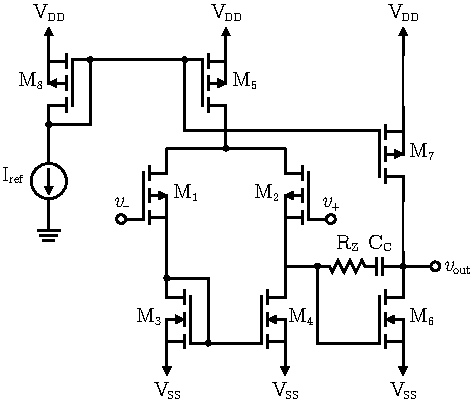
\includegraphics[width=6cm]{circuits/op_amp_schematic.pdf}
				\caption{Τελεστικός ενισχυτής δύο σταδίων. Στην έξοδο του ενισχυτή συνδέεται χωρητικό φορτίο $C_L$. Όλα τα transistor λειτουργούν στην περιοχή κορεσμού.}
				\label{circ:op_amp_schematic}
			\end{circuitfig}
		\end{center}
		
Οι προδιαγραφές του ζητούμενου τελεστικού ενισχυτή δίδονται στον πίνακα \ref{table:specs}.

\begin{table}[H]
	\begin{center}
		\begin{tabular}{|r|l|}
			\hline
			\multirow[|r|]{2}{*}{\textbf{Τροφοδοσία}}           & $V_{SS} =-2.31\unit{\volt}$                         \\\cline{2-2}
			                                                    & $V_{DD} =+2.31\unit{\volt}$                         \\\hline
			\multirow[|r|]{2}{*}{\textbf{Εύρος τάσεως εισόδου}} & $\min{\(v_{\mathrm{in}}\)} =-100\unit{\milli\volt}$ \\\cline{2-2}
			                                                    & $\max{\(v_{\mathrm{in}}\)} =+100\unit{\milli\volt}$ \\\hline
			\textbf{Κέρδος τάσεως}                              & $A_v >20.17\unit{\decibel}$                         \\\hline
			\textbf{Καταναλισκόμενη ισχύς}                      & $P_\mathrm{diss} <50.17\unit{\milli\watt}$          \\\hline
			\textbf{Gain bandwidth}                             & $\GB >7.17\unit{\mega\hertz}$                       \\\hline
			\textbf{Slew rate}                                  & $\SR >18.17\,\unit{\volt\per{\micro\sec}}$          \\\hline
			\textbf{Χωρητικότητα φορτίου}                       & $C_L =2.17\unit{\pico\farad}$                       \\\hline
		\end{tabular}
		\caption{Προδιαγραφές και δεδομένα για τον τελεστικό ενισχυτή του κυκλώματος \ref{circ:op_amp_schematic}.}
		\label{table:specs}
	\end{center}
\end{table}
		\section{Χαρακτηριστικά των transistor}
	Οι τιμές των παραμέτρων προσδιορίσθηκαν μέσω των μοντέλων PSpice των transistor της εκφώνησης, παραρτήματα \ref{appendix:pspice_models_pmos} και \ref{appendix:pspice_models_nmos}. Στα μοντέλα έχει προστεθεί και η παράμετρος \texttt{L=1u} η οποία αντιστοιχεί στο μήκος του διαύλου.\par

	\subsection{pMOS}
	Τα MOSFET διαύλου p έχουν τάση κατωφλίου $V_{T0,p}=-0.9056\unit{\volt}$. Η παράμετρος διαγωγιμότητάς \textsl{(process transconductance parameter)} τους είναι $k_p^\prime=\mu_p\cdot C_{ox,p}=2.9352\cdot 10^{-5}\unit{\ampere\per{\volt^2}}$, όπου $C_{ox,p}$ είναι η χωρητικότητα του στρώματος οξειδίου \textsl{(oxide capacitance)} και $\mu_p=180.2\unit{{\centi\meter}^2\per{\volt\sec}}$ η κινητικότητα των οπών στον δίαυλο.\cite{sedra} Το πάχος του στρώματος του οξειδίου είναι $t_{ox,p}=21.2\unit{\nano\meter}$. Από τα παραπάνω εύκολα προκύπτει πως η χωρητικότητα του στρώματος οξειδίου είναι $C_{ox,p}=\sfrac{k_p^\prime}{\mu_p}=134.642\unit{\micro\farad\per{\centi\meter}^2}$.

\subsection{nMOS}
	Τα MOSFET διαύλου n έχουν τάση κατωφλίου $V_{T0,n}=0.7860\unit{\volt}$. Το process transconductance parameter τους δίδεται $k_n^\prime=\mu_n\cdot C_{ox,n}=9.6379\cdot 10^{-5}\unit{\ampere\per{\volt^2}}$, όπου $C_{ox,n}$ είναι η χωρητικότητα του στρώματος οξειδίου \textsl{(oxide capacitance)} και $\mu_n=591.7\unit{{\centi\meter}^2\per{\volt\sec}}$ η κινητικότητα των ηλεκτρονίων στον δίαυλο.\cite{sedra} Το πάχος του στρώματος του οξειδίου είναι $t_{ox,n}=21.2\unit{\nano\meter}$. Από τα παραπάνω εύκολα προκύπτει πως η χωρητικότητα του στρώματος οξειδίου είναι $C_{ox,p}=\sfrac{k_p^\prime}{\mu_p}=0.162\:885\unit{\micro\farad\per{\centi\meter}^2}$.
		\section{Εκτίμηση aspect ratio $\displaystyle{S=\sfrac{W}{L}}$ των transistor}
\subsection{Θεωρητική ανάλυση}
Η χωρητικότητα Miller, $C_C$, στο κύκλωμα \ref{circ:op_amp_schematic} εξασφαλίζει πως η συχνότητα $\omega_{p_1}$ του πόλου $p_1$ της συνάρτησης μεταφοράς του ενισχυτή μετατοπίζεται σε συχνότητες κοντά στο μηδέν και η συχνότητα $\omega_{p_2}$ του πόλου $p_2$ μετατοπίζεται σε υψηλότερες συχνότητες. Έστω, $p_1\to 0$ και $\omega_Z=10\cdot \mathrm{GB}$, τότε, εάν το περιθώριο φάσης είναι $60^\circ$, θα έχουμε

\begin{align*}
	 & \phi_M=180^\circ-\arctan{\(\frac{\mathrm{GB}}{\omega_{p_1}}\)}-\arctan{\(\frac{\mathrm{GB}}{\omega_{p_2}}\)}-\arctan{\(\frac{\mathrm{GB}}{\omega_{Z}}\)}\Rightarrow \\
	 & 60^\circ=180^\circ-90^\circ-\arctan{\(\frac{\mathrm{GB}}{\omega_{p_2}}\)}-\arctan{\(0.1\)}\Rightarrow                                                               \\
	 & \omega_{p_2}=2.215\cdot\mathrm{GB}.
\end{align*}
Από τη συνθήκη $\omega_Z=10\cdot \mathrm{GB}$ προκύπτει
\begin{equation*}
	\omega_Z=\frac{g_{m6}}{C_C}\Rightarrow 10\cdot \mathrm{GB}=\frac{g_{m6}}{C_C}\Rightarrow 10\cdot\frac{g_{m1}}{C_C}=\frac{g_{m6}}{C_C}
\end{equation*}
δηλαδή
\begin{equation}
	g_{m6}=10\cdot g_{m1}.
\end{equation}

Από το περιθώριο φάσης προέκυψε $\omega_{p_2}>2.215\cdot\mathrm{GB}$. Επομένως, είναι
\begin{align*}
	 & \omega_{p_2}>2.215\cdot\mathrm{GB}\Rightarrow\frac{g_{m6}}{C_L}>2.215\cdot\mathrm{GB}\Rightarrow \\
	 & 10\frac{g_{m1}}{C_L}>2.215\cdot\frac{g_{m1}}{C_C}
\end{align*}
ή
\begin{equation}
	C_C>0.222\cdot C_L
\end{equation}

Από το slew rate μπορεί να εκτιμηθεί το ρεύμα $I_{D5}$ ως εξής
\begin{equation}
	\mathrm{SR}=\frac{I_{D5}}{C_C}\Rightarrow I_{D5}=\mathrm{SR}\cdot C_C
\end{equation}
Θεωρώντας πως $I_{D5}=2\cdot I_{D1}=2\cdot{I_{D3}}$ και πως τα M1---M2 και M3---M4 είναι πανομοιότυπα, έχουμε
\begin{align}
	S_3=\frac{I_{D5}}{k_n^\prime\cdot\(\min{\(v_{\mathrm{in}}\)}-V_{SS}+|V_{T0,1p}|-V_{T0,3n}\)^2}
\end{align}
Θα είναι $S_3=S_4$ και εφόσον όλα τα transistor έχουν μήκος διαύλου $L=1\unit{\micro\meter}$, θα έχουν πλάτος διαύλου $W_3=W_4=S_3\unit{\micro\meter}$.

Έπειτα, εξετάζεται εάν η συχνότητα του πόλου $p_3$ είναι μεγαλύτερη από $10\cdot \mathrm{GB}$. Είναι
\begin{equation*}
	\omega_{p_3}=\frac{g_{m_3}}{2C_{gs3}}=\frac{\sqrt{2\cdot k_n^\prime\cdot S_3\cdot I_{D3}}}{0.667\cdot W_3\cdot L_3\cdot C_{ox,n}}
\end{equation*}
ή
\begin{equation}
	\omega_{p_3}=\frac{\sqrt{k_n^\prime\cdot S_3\cdot I_{D5}}}{0.667\cdot S_3\cdot L_3^2\cdot C_{ox,n}}
\end{equation}

Η διαγωγιμότητα των transistor M1 και M2 υπολογίζεται μέσω του gain-bandwidth product. Είναι $g_{m1}=g_{m2}=\mathrm{GB}\cdot C_C$. Το aspect ratio τους είναι
\begin{equation}
	S_1=S_2=\frac{g_{m1}^2}{k_p^\prime\cdot I_{D5}}.
\end{equation}

Εν συνεχεία υπολογίζεται το $S_5$.
\begin{equation}
	S_5=\frac{2\cdot I_{D5}}{k_p^\prime\cdot V_{DS5,\mathrm{sat}}^2},
\end{equation}
όπου
\begin{equation}
	V_{DS5,\mathrm{sat}}=\max\(v_{\mathrm{in}}\)-V_{DD}+\sqrt{\frac{I_{D5}}{\beta_1}}+|V_{T0,p}|
\end{equation}
και
\begin{equation}
	\beta_1=k_p^\prime\cdot S_1.
\end{equation}

Για το transistor M6 έχουμε
\begin{equation}
	S_6=S_4\cdot\frac{g_{m6}}{g_{m4}},
\end{equation}
όπου
\begin{equation}
	g_{m4}=\sqrt{2\cdot k_n^\prime\cdot S_4\cdot I_{D4}}.
\end{equation}

Τέλος, το $S7$ μπορεί να υπολογιστεί είτε μέσω της σχέσης \eqref{eq:S7a} είτε μέσω της \eqref{eq:S7b}. Εδώ επιλέγεται η σχέση \eqref{eq:S7a} η οποία, σε θεωρητικό επίπεδο, εξασφαλίζει την απουσία συστηματικού dc offset.\cite{sedra}
\begin{equation}
	\label{eq:S7a}
	S_7=2\frac{S_6\cdot S_5}{S_4}.
\end{equation}
Εναλλακτικά,
\begin{equation}
	\label{eq:S7b}
	S_7=S_5\frac{I_{D7}}{I_{D5}},
\end{equation}
όπου
\begin{equation}
	I_{D6}=I_{D7}=\frac{g_{m6}^2}{2\cdot k_n^\prime\cdot S_6}.
\end{equation}

\subsection{Αποτελέσματα εκτίμησης}
Όλα τα παραπάνω εφαρμόζονται στο matlab script \texttt{op\_amp\_S.m}. Τα αποτελέσματα δίδονται στον πίνακα \ref{table:estimate}.

\begin{table}[H]
	\begin{center}
		\begin{tabular}{|l|l|}
			\hline
			\multicolumn{2}{|c|}{\textbf{Aspect ratios}}                        \\\hline
			$S_1 = 1.816719$             & $S_5 = 3.024399$                     \\\hline
			$S_2 = 1.816719$             & $S_6 = 37.567524$                    \\\hline
			$S_3 = 25.508331$            & $S_7 = 8.908399$                     \\\hline
			$S_4 = 25.508331$            & $S_8 = 3.024399$                     \\\hline\hline
			\textbf{Χωρητικότητα Miller} & $C_C=0.4774\unit{\pico\farad}$       \\\hline
			\textbf{Αντίσταση μηδενικού} & $R_Z=46.496318\kohm$                 \\\hline
			\textbf{Ρεύμα εκροής του M5} & $I_5 = 8.674358\unit{\micro\ampere}$ \\\hline
		\end{tabular}
		\caption{Εκτίμηση των παραμέτρων του κυκλώματος \ref{circ:op_amp_schematic}. Το αναμενόμενο κέρδος τάσης ανοιχτού βρόχου είναι $A_v=196.96$ και η κατανάλωση ισχύος αναμένεται $P_{\mathrm{diss}}=0.056\unit{\milli\watt}$.}
		\label{table:estimate}
	\end{center}
\end{table}
		\section{Προσομοίωση}
Το κυκλώματα με τις τιμές των παραμέτρων του πίνακα \ref{table:estimate}, όταν προσομοιώθηκε, δεν πληρούσε την προδιαγραφές για gain-bandwidth product και το περιθώριο φάσης. Το κέρδος ανοιχτού βρόχου πληρεί την προδιαγραφή του πίνακα \ref{table:specs}.\par

\subsection{Ρυθμίσεις}
Το κέρδος τάσης ανοιχτού βρόχου δίνεται από την έκφραση
\begin{equation}
	\label{eq:Av}
	A_v=\frac{2\cdot g_{m1}\cdot g_{m6}}{I_{D5}\(\lambda_2+\lambda_5\)\cdot I_{D6}\(\lambda_6+\lambda_7\)}.
\end{equation}

Επιπλέον, για το διαφορικό ζεύγος απαιτείται υψηλή διαγωγιμότητα προκειμένου να μειώνεται η συνεισφορά του θερμικού θορύβου,\cite{lectureSlides} οπότε αυξάνονται οι λόγοι $S_1$ και $S_2$. Αυτό οδηγεί σε μία αύξηση του κέρδους ανοιχτού βρόχου, παρόλο που ήταν ήδη εντός των προδιαγραφών.

Το gain-bandwidth product δίνεται από την έκφραση
\begin{equation}
	\mathrm{GB}=A_v(0)\cdot|\omega_{p_1}|=\frac{g_{m1}}{C_C}.
\end{equation}
Αυτό σημαίνει πως η αύξηση των $S_1$ και $S_2$ βελτιώνει και το gain-bandwidth το οποίο επιβεβαιώνεται και από το την προσομοίωση. Τα $g_{m1}$, $g_{m2}$ μπορούν να αυξηθούν και μέσω της αύξησης του $I_{D5}=\sfrac{I_{D1}}{2}$ το οποίο όμως, εξαιτίας της σχέσης \ref{eq:Av}, φαίνεται να μειώνει το κέρδος ανοιχτού βρόχου. To $I_{D5}$ αυξάνεται μέσω της αύξησης του $I_{\mathrm{ref}}$. Με αύξηση του $S_5$ στο δεκαπλάσιο της αρχικής του τιμής, το $I_{D5}$ φαίνεται να δεκαπλασιάζεται και αυτό με αντίκτυπο στο κέρδος ανοιχτού βρόχου το οποίο όμως παραμένει εντός των προδιαγραφών.\par
Επιπλέον, η αύξηση, κατά περίπου $4.4$ φορές, του $S_7$ και κατά συνέπεια του $I_{D7}=I_{D6}$ αν και αναμένεται να μειώσει το κέρδος ανοιχτού βρόχου, έχει μικρή επίδραση σε κλίμακα decibel. Ωστόσο, βελτιώνει σημαντικά το gain-bandwidth product.\par
Το $S_6$ μειώνεται στην μισή τιμή του νέου $S_7$ το οποίο αν και επιδρά αρνητικά στο κέρδος, αυξάνει (προς το μηδέν) την φάση της εξόδου.\par
Η αντίσταση $R_Z$ παίρνει τιμή αρκετά μεγαλύτερη της $\frac{1}{g_{m2}}$ που απαιτείται για την μετατόπιση του μηδενικού σε \textsl{άπειρη} συχνότητα.\cite{sedra} Χρησιμοποιώντας τιμή μεγαλύτερη της $\frac{1}{g_{m2}}$ το μηδενικό μετατοπίζεται στον αρνητικό πραγματικό ημιάξονα και αυξάνει το περιθώριο φάσης.\cite{sedra}\par
Για τη μείωση της κατανάλωσης ισχύος χωρίς να επηρεασθούν σημαντικά οι υπόλοιπες παράμετροι του ενισχυτή, αυξάνεται ελαφρώς, κατά $3\unit{\micro\meter}$, ο λόγος $S_8$.\par
Τέλος, οι λόγοι $S_3$, $S_4$ ρυθμίζονται βάση της σχέσης \eqref{eq:S7a}.\par

Οι προσομοιώσεις έγιναν με το κύκλωμα \ref{circ:op_amp_sim}. Στο κύκλωμα \ref{circ:op_amp_sources} φαίνονται οι πηγές τροφοδοσίας και οι πηγές που εφαρμόζονται στην μη αναστρέφουσα είσοδο για έλεγχο των προδιαγραφών. Η αναστρέφουσα είσοδος συνδέεται μέσω του βρόχου ανάδρασης του κυκλώματος \ref{circ:op_amp_feedback_loop} στην έξοδο του ενισχυτή. \par

\begin{center}
	\begin{circuitfig}[H]
		\centering
		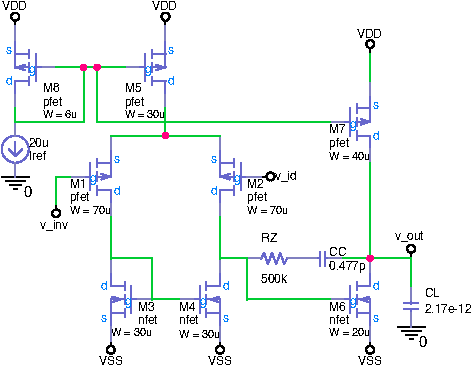
\includegraphics[width=8cm]{op_amp_sim/op_amp_main.pdf}
		\caption{CMOS τελεστικός ενισχυτής δύο σταδίων.Τα μήκη των διαύλων όλων των transistor είναι $L=1\unit{\micro\meter}$ και τα πλάτη αναγράφονται δίπλα στο κάθε transistor.}
		\label{circ:op_amp_sim}
	\end{circuitfig}
	\begin{circuitfig}[H]
		\centering
		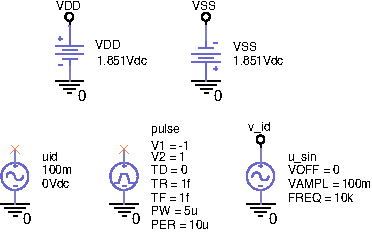
\includegraphics[width=6.3cm]{op_amp_sim/op_amp_sources.pdf}
		\caption{Η πηγή τάσης \texttt{uid} χρησιμοποιείται για την παραγωγή διαγράμματος Bode. Η πηγή \texttt{u\_sin} χρησιμοποιείται στην ανάλυση στο πεδίο του χρόνου (transient analysis) και η πηγή \texttt{pulse} παράγει τετραγωνικό παλμό για την μέτρηση του slew rate.}
		\label{circ:op_amp_sources}
	\end{circuitfig}
	\begin{circuitfig}[H]
		\centering
		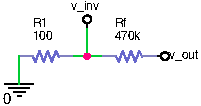
\includegraphics[width=3.5cm]{op_amp_sim/op_amp_feedback_loop.pdf}
		\caption{Δίκτυο ανάδρασης. Η τιμή της $R_f$ δεν μπορεί να είναι πολύ υψηλή διότι θα αυξηθεί η κατανάλωση ισχύος. Λόγω της μεγάλης τιμής της $R_f$ και της μικρής τιμής της $R_1$ η τάση στην αναστρέφουσα είσοδο του τελεστικού είναι πολύ κοντά στη γείωση, της τάξεως λίγων εκατοντάδων $\unit{\micro\volt}$ (κύκλωμα \ref{circ:op_amp_labels}).}
		\label{circ:op_amp_feedback_loop}
	\end{circuitfig}
\end{center}
% \vspace*{-0.5cm}

\subsection{Συχνοτική απόκριση}
% Το κέρδος ανοιχτού βρόχου και η φάση της εξόδου του κυκλώματος \ref{circ:op_amp_schematic} φαίνονται στο διάγραμμα \ref{plot:bode}.

\begin{center}
	\begin{plotenv}[H]
		\centering
		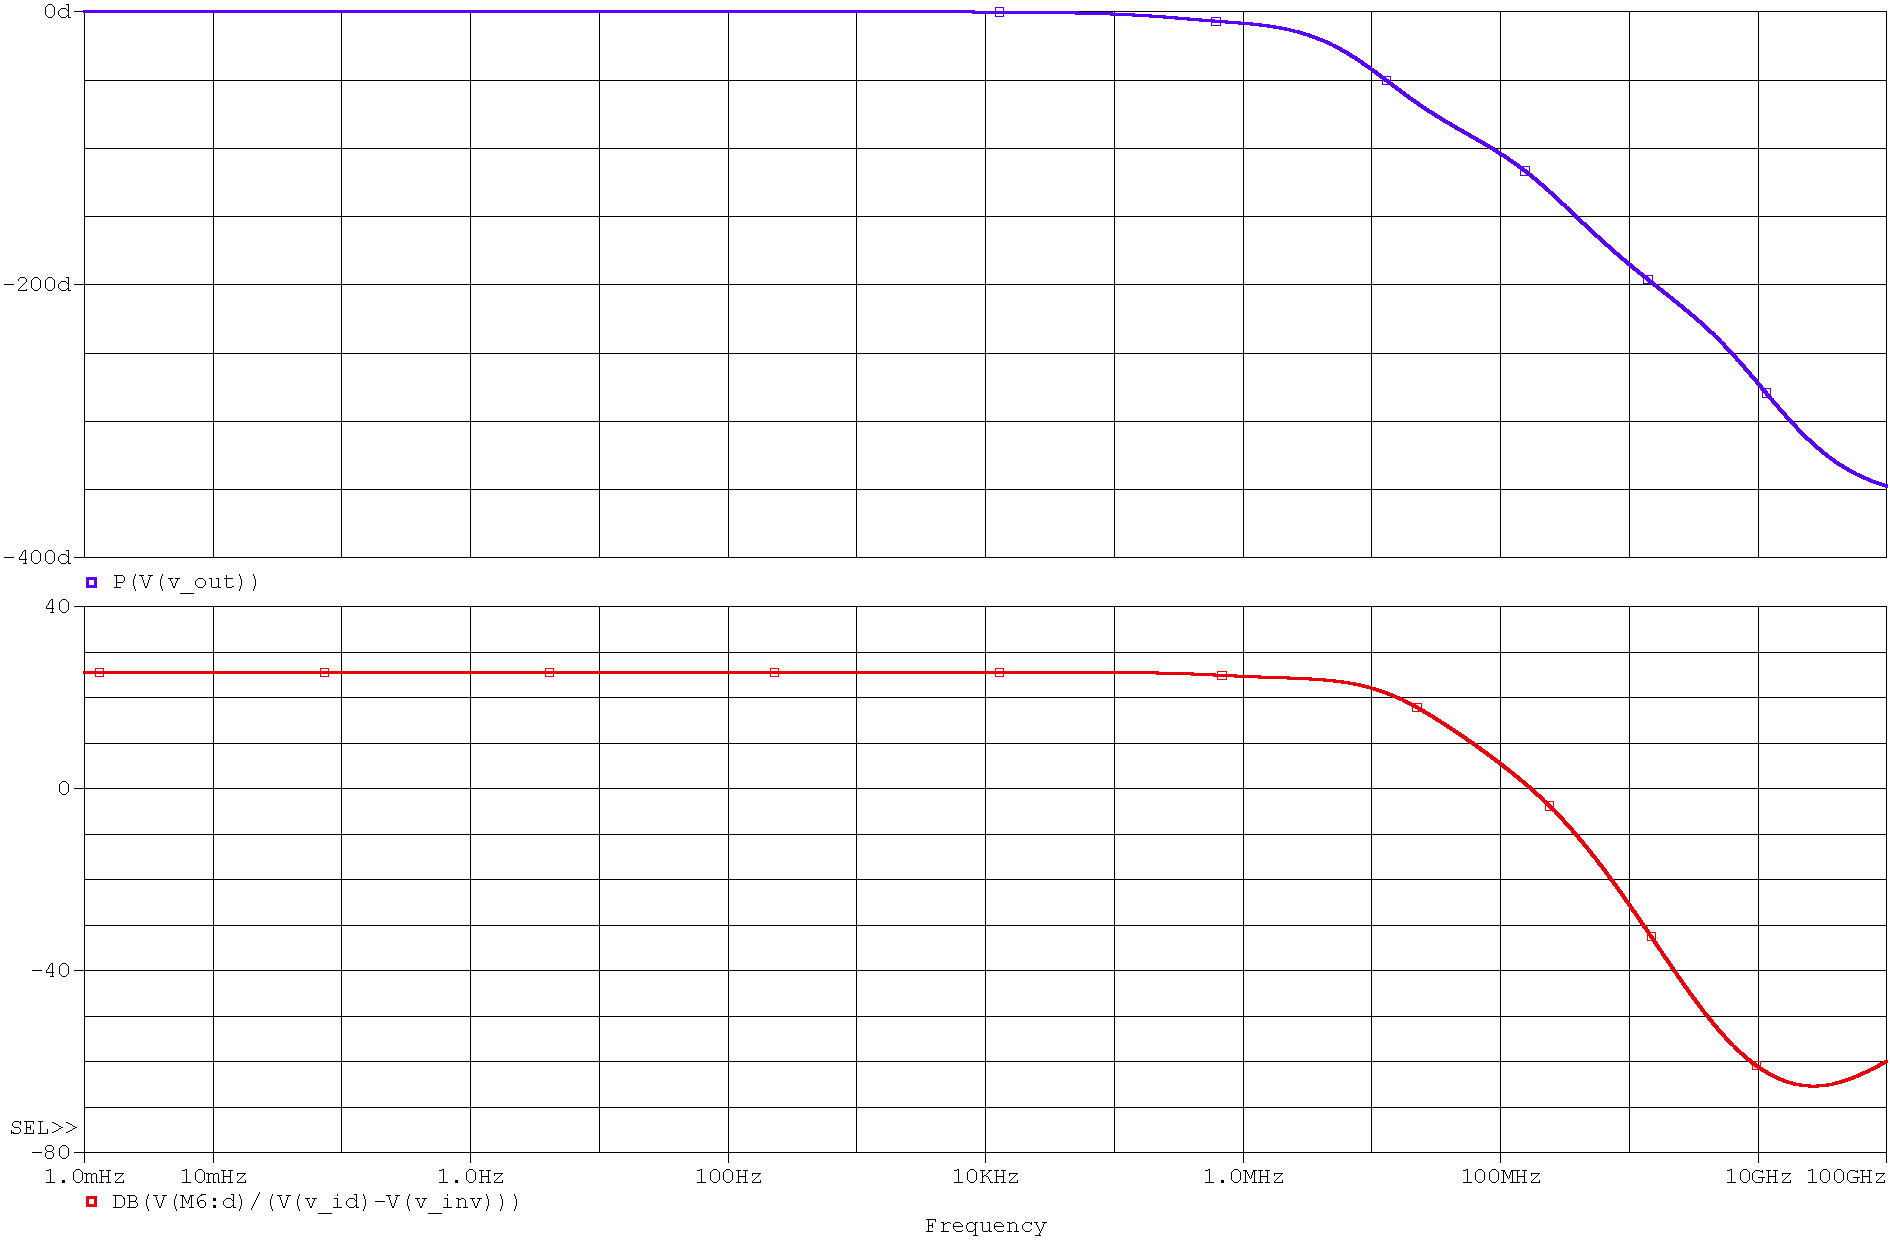
\includegraphics[width=\linewidth]{op_amp_sim/bode.pdf}
		\caption{Με κόκκινο χρώμα διαγράφεται το κέρδος τάσης εξόδου σε $\unit{\decibel}$ και με μπλε χρώμα διαγράφεται η φάση της εξόδου.}
		\label{plot:bode}
	\end{plotenv}
\end{center}
\vspace*{-0.5cm}

Το μέγιστο του κέρδους τάσης στο πεδίο της συχνότητας βρέθηκε στα $20\cdot\log_{10}{A_v}=25.55619$.\par
Το gain-bandwidth product εκτιμήθηκε στο σημείο όπου η καμπύλη του κέρδους σημειώνει μείωση κατά $3\unit{\decibel}$ από την σταθερή τιμή της και βρέθηκε $\mathrm{GB}=8.70313\unit{\mega\hertz}$.\par
Το περιθώριο φάσης βρέθηκε $\phi_M=59.95727^\circ$. Συγκεκριμένα, το περιθώριο φάσης ισούται με το άθροισμα της φάσης της εξόδου στη συχνότητα μοναδιαίου κέρδους (unity gain frequency) και των $180^\circ$.\par
Στον πίνακα \ref{table:gb_measurements} παρατίθενται οι εκφράσεις που χρησιμοποιήθηκαν στο PSpice για τον προσδιορισμό των παραπάνω και το αποτέλεσμά τους.\par
\begin{table}[H]
	\begin{center}
		\begin{tabular}{|c|l|}
			\hline
			\footnotesize{\textbf{Μέγεθος}}                      & \footnotesize{\textbf{PSpice measurement expression}}                        \\\hline\hline
			\tiny{$20\log{(A_v)} \left[\unit{\decibel}\right]$}  & \tiny{\texttt{Max(DB(V(M6:d)/(V(v\_id)-V(v\_inv))))}}                        \\\hline
			\tiny{$\mathrm{GB} \left[\unit{\mega\hertz}\right]$} & \tiny{\texttt{PhaseMargin(DB(V(v\_out)/(V(v\_id)-V(v\_inv))),P(V(v\_out)))}} \\\hline
			\tiny{$\phi_M \left[{}^\circ\right]$}                & \tiny{\texttt{Cutoff\_Lowpass\_3dB(DB(V(v\_out)/(V(v\_id)-V(v\_inv))))}}     \\\hline
		\end{tabular}
		\caption{PSpice measurements για τον υπολογισμό του κέρδους ανοιχτού βρόχου, gain-bandwidth product και του περιθωρίου φάσης της εξόδου.}
		\label{table:gb_measurements}
	\end{center}
\end{table}


\subsection{Κατανάλωση ισχύος}
Η κατανάλωση ισχύος εκτιμάται μέσω transient analysis σε διάστημα μίας περιόδου με ημιτονοειδές σήμα πλάτους $200\unit{\milli\volt}_\mathrm{pp}$ συχνότητας $10\unit{\kilo\hertz}$ συνδεδεμένο στη μη αναστρέφουσα είσοδο του ενισχυτή.\par
Πρώτος τρόπος εκτίμησης είναι μέσω των bias currents του κυκλώματος \ref{circ:op_amp_labels}. Συγκεκριμένα, η κατανάλωση ισχύος θα είναι
\begin{align*}
	P_\mathrm{diss}= & \(|I_{D5}|+|I_{D6}|+|I_{D8}|\)\cdot\(V_{DD}+|V_{SS}|\)                            \\
	=                & \(95.51+144.50+20.00\)\cdot\(1.851+1.851\)\;\unit{\micro\ampere}\cdot\unit{\volt} \\
	=                & 0.963\unit{\milli\watt}\ll 50.17\unit{\milli\watt}.
\end{align*}

\begin{circuitfig}[H]
	\centering
	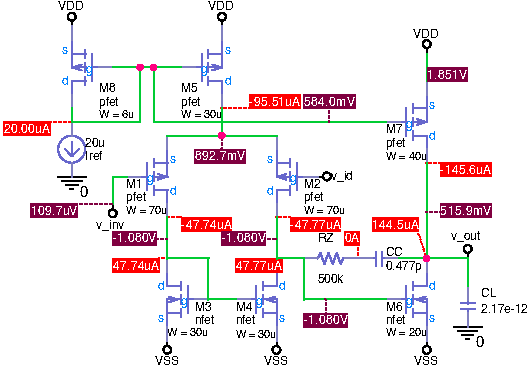
\includegraphics[width=9cm]{op_amp_sim/op_amp_labels.pdf}
	\caption{Bias τάσεις και εντάσεις ρευμάτων για $u_+$ πλάτους $200\unit{\milli\volt}_\mathrm{pp}$ συχνότητας $10\unit{\kilo\hertz}$.}
	\label{circ:op_amp_labels}
\end{circuitfig}

Ο δεύτερος τρόπος είναι η ανάγνωση της τιμής από το output αρχείο της προσομοίωσης, \texttt{trans.out} στην προκειμένη. Ειδικότερα, η κατανάλωση ισχύος είναι $0.928\unit{\milli\watt}$ όπως φαίνεται από το παρακάτω χωρίο του \texttt{trans.out}.\par
\footnotesize{\begin{verbatim}
	VOLTAGE SOURCE CURRENTS
	NAME         CURRENT

	V_uid        0.000E+00
	V_VSS       -2.400E-04
	V_pulse      0.000E+00
	V_VDD       -2.611E-04
	V_u_sin      0.000E+00

	TOTAL POWER DISSIPATION   9.28E-04  WATTS
\end{verbatim}}

\subsection{Slew rate}
Για τον υπολογισμό του slew rate, κατά τις οδηγίες της εκφώνησης, στην μη αναστρέφουσα είσοδο του ενισχυτή εφαρμόσθηκε τετραγωνικός παλμός πλάτους $1\unit{\volt}$. Παρακολουθείται η έξοδος σε θετική ακμή του παλμού της εισόδου. Βρίσκεται η χρονική στιγμή κατά την οποία η έξοδος είναι στο $10\%$ του πλάτους της peak to peak και βρίσκεται και η χρονική στιγμή κατά την οποία η έξοδος είναι στο $90\%$ του πλάτους της peak to peak. Το slew rate θα είναι ο λόγος $\mathrm{SR}=\displaystyle{\frac{u_{0.9}-u_{0.1}}{t_{0.9}-t_{0.1}}}$.\par
Το PSpice παρέχει τη συνάρτηση \texttt{SlewRate\_Rise($\cdot$)} η οποία ακολουθεί την παραπάνω διαδικασία αλλά στο $25\%$ και στο $75\%$ του πλάτους της peak to peak αντί για $10\%$ και $90\%$ αντιστοίχως. Για τον λόγο αυτό, με βάση την \texttt{SlewRate\_Rise($\cdot$)} δημιουργήθηκε μία νεα συνάρτηση \texttt{SlewRate\_Rise\_M($\cdot$)} η οποία περιγράφεται στο αρχείο \texttt{\textbackslash op\_amp\textbackslash op\_amp-PSpiceFiles\textbackslash SCHEMATIC1\textbackslash slew\_rate\textbackslash slew\_rate.prb}. Παρακάτω παρατίθεται ο κώδικάς της.\par
\footnotesize{\begin{verbatim}
SlewRate_Rise_M(1)=(y4-y3)/(x4-x3)
   {
      1|Search forward x value (0%) !1
	Search forward x value (100%) !2
	Search forward /Begin/ level (y1+0.1*(y2-y1),p) !3
	Search forward level (y1+0.9*(y2-y1),p) !4;
   }
\end{verbatim}}

Το αποτέλεσμα της μέτρησης είναι $\mathrm{SR}=69.20035\;\unit{\volt\per{\micro\second}}$, πολύ μεγαλύτερο από το ελάχιστο όριο που απαιτείται, $18.17\;\unit{\volt\per{\micro\second}}$.\par

\begin{center}
	\begin{plotenv}[H]
		\centering
		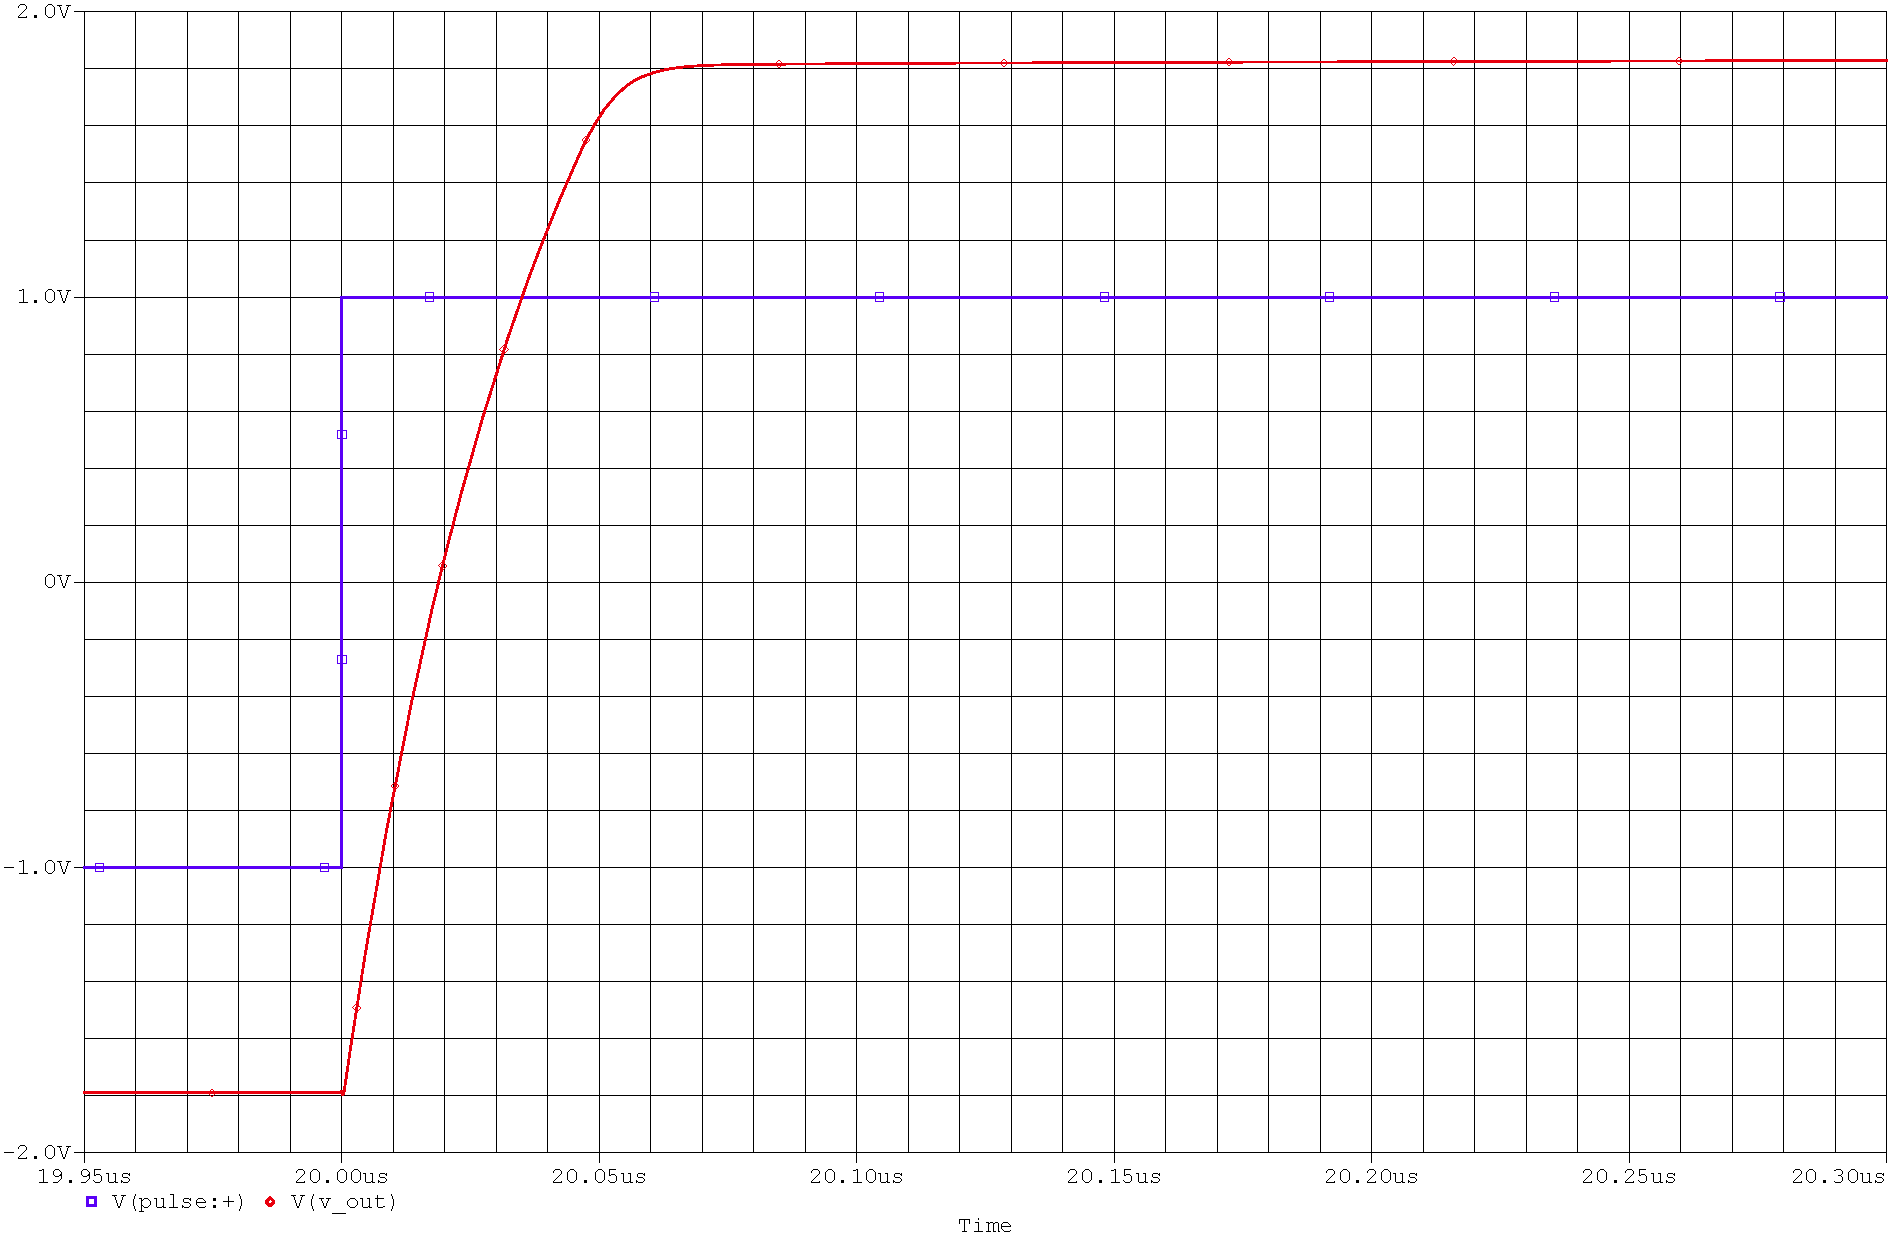
\includegraphics[width=\linewidth]{op_amp_sim/slew_rate.pdf}
		\caption{Με κόκκινο χρώμα διαγράφεται η έξοδος του τελεστικού ενισχυτή και με μπλε χρώμα διαγράφεται ο τετραγωνικός παλμός πλάτους $1\unit{\volt}$ που εφαρμόζεται στην μη αναστρέφουσα είσοδό του.}
		\label{plot:slew_rate}
	\end{plotenv}
\end{center}

% \vspace*{-0.5cm}
\subsection{Temperature sweep}

Όλες οι παραπάνω προσομοιώσεις επαναλήφθηκαν σε θερμοκρασίες $-20\unit{\celsius}$, $0\unit{\celsius}$, $20\unit{\celsius}$, $40\unit{\celsius}$, $60\unit{\celsius}$, $80\unit{\celsius}$ και $100\unit{\celsius}$. Στον πίνακα \ref{table:measurements_temp} δίνονται οι μετρήσεις των κυματομορφών. Η κατανάλωση ισχύος βρέθηκε μέσω των output αρχείων των παραμετρικών προσομοιώσεων.\par

\begin{table}[H]
	\begin{center}
		\footnotesize{\begin{tabular}{|r|c|c|c|c|}
				\hline
				\textbf{Μέγεθος}                                 & $\mathbf{-20\unit{\celsius}}$ & $\mathbf{0\unit{\celsius}}$ & $\mathbf{20\unit{\celsius}}$ & $\mathbf{27\unit{\celsius}}$ \\\hline\hline
				$20\cdot\log_{10}{\(A_v\)}\;[\unit{\decibel}]$   & $25.53643$                    & $25.54701$                  & $25.55431$                   & $25.55619$                   \\\hline
				$\mathrm{GB}\;[\unit{\mega\hertz}]$              & $10.51383$                    & $9.67467$                   & $8.93937$                    & $8.70313$                    \\\hline
				$\phi_M$                                         & $59.09589^\circ$              & $59.46750^\circ$            & $59.83206^\circ$             & $59.95727^\circ$             \\\hline
				$P_{\mathrm{diss}}\;[\unit{\milli\watt}]$        & $0.944$                       & $0.936$                     & $0.930$                      & $0.928$                      \\\hline
				$\mathrm{SR}\;[\unit{\volt\per{\micro\second}}]$ & $70.59513$                    & $69.69387$                  & $68.93170$                   & $69.20035$                   \\\hline
			\end{tabular}}
		\end{center}

		\begin{center}
		\footnotesize{\begin{tabular}{|r|c|c|c|c|}
				\hline
				\textbf{Μέγεθος}                                 & $\mathbf{40\unit{\celsius}}$ & $\mathbf{60\unit{\celsius}}$ & $\mathbf{80\unit{\celsius}}$             & $\mathbf{100\unit{\celsius}}$            \\\hline\hline
				$20\cdot\log_{10}{\(A_v\)}\;[\unit{\decibel}]$   & $25.55887$                   & $25.56106$                   & $28.67671$                               & $28.70726$                               \\\hline
				$\mathrm{GB}\;[\unit{\mega\hertz}]$              & $8.29010$                    & $7.71244$                    & \textcolor{IndianRed2}{$6.15171$}        & \textcolor{IndianRed2}{$5.65827$}        \\\hline
				$\phi_M$                                         & $60.18563^\circ$             & $60.52578^\circ$             & \textcolor{IndianRed2}{$44.59798^\circ$} & \textcolor{IndianRed2}{$44.73339^\circ$} \\\hline
				$P_{\mathrm{diss}}\;[\unit{\milli\watt}]$        & $0.924$                      & $0.920$                      & $0.916$                                  & $0.913$                                  \\\hline
				$\mathrm{SR}\;[\unit{\volt\per{\micro\second}}]$ & $68.69967$                   & $67.64329$                   & $67.17787$                               & $66.42879$                               \\\hline
			\end{tabular}}
		\end{center}
		\centering
		\caption{Μετρήσεις των παραμέτρων των προδιαγραφών για τις θερμοκρασίες $-20\unit{\celsius}$, $0\unit{\celsius}$, $20\unit{\celsius}$ και $27\unit{\celsius}$.}
		\label{table:measurements_temp}
\end{table}

Από τα δεδομένα του πίνακα \ref{table:measurements_temp} φαίνεται πως στους $80\unit{\celsius}$ και $100\unit{\celsius}$ το $\mathrm{GB}$ είναι σημαντικά χαμηλότερο της προδιαγραφής ενώ το περιθώριο φάσης είναι μόλις $0.4^\circ$ και $0.3^\circ$ κάτω των $45^\circ$ αντίστοιχα.\par

\begin{plotenv}[H]
	\centering
	\begin{tikzpicture}
		\begin{axis}[
				height=5cm,
				width=\linewidth,
				xlabel={Temperature [$\unit{\celsius}$]},
				legend style={at={(0.032,+1.025)},anchor=south west,legend columns=3},
				ymajorgrids=true,
				xmajorgrids=true,
				grid style=dashed,
				ytick=\empty
			]
			\addplot[color=IndianRed2,mark=square,thick]
			coordinates {
					(-20,25.53643)
					(0,25.54701)
					(20,25.55431)
					(27,25.55619)
					(40,25.55887)
					(60,25.56106)
					(80,28.67671)
					(100,28.70726)
				};
			\addlegendentry{$20\cdot\log_{10}{\(A_v\)}\;[\unit{\decibel}]$}

			\addplot[color=SeaGreen3,mark=*,thick]
			coordinates {
					(-20,10.51383)
					(0,9.67467)
					(20,8.93937)
					(27,8.70313)
					(40,8.29010)
					(60,7.71244)
					(80,6.15171)
					(100,5.65827)
				};
			\addlegendentry{$\mathrm{GB}\;[\unit{\mega\hertz}]$}

			\addplot[color=SlateBlue3,mark=triangle,thick]
			coordinates {
					(-20,59.09589)
					(0,59.46750)
					(20,59.83206)
					(27,59.95727)
					(40,60.18563)
					(60,60.52578)
					(80,44.59798)
					(100,44.73339)
				};
			\addlegendentry{$\phi_M$}

			\addplot[color=Turquoise4,mark=diamond,thick]
			coordinates {
					(-20,0.944)
					(0,0.936)
					(20,0.930)
					(27,0.928)
					(40,0.924)
					(60,0.920)
					(80,0.916)
					(100,0.913)
				};
			\addlegendentry{$P_{\mathrm{diss}}\;[\unit{\milli\watt}]$}

			\addplot[color=PaleVioletRed3,mark=pentagon,thick]
			coordinates {
					(-20,70.59513)
					(0,69.69387)
					(20,68.93170)
					(27,69.20035)
					(40,68.69967)
					(60,67.64329)
					(80,67.17787)
					(100,66.42879)
				};
			\addlegendentry{$\mathrm{SR}\;[\unit{\volt\per{\micro\second}}]$}
		\end{axis}
	\end{tikzpicture}
	\caption{Ποιοτική μεταβολλή των παραμέτρων $A_v$, $\mathrm{GB}$, $\phi_M$, $P_\mathrm{diss}$ και $\mathrm{SR}$ συναρτήσει της θερμοκρασίας.}
	\label{plot:parameter_temp}
\end{plotenv}

Από τα δεδομένα του πίνακα \ref{table:measurements_temp} και το διάγραμμα \ref{plot:parameter_temp} παρατηρείται πως τα μόνα μεγέθη με γνησίως καθοδική πορεία είναι το slew rate και το gain-bandwidth product.\par
Το gain-bandwidth product παρουσιάζει μία σχεδόν γραμμική μείωση με την αύξηση της θερμοκρασίας. Στους $80\unit{\celsius}$ βγαίνει εκτός προδιαγραφών κατά περίπου $1\unit{\mega\hertz}$.\par
Στην κατανάλωση ισχύος, παρατηρείται μία μικρή αύξηση με την άνοδο της θερμοκρασίας και η διαφορά μεταξύ των $-20\unit{\celsius}$ και των $100\unit{\celsius}$ είναι $31\unit{\micro\watt}$.\par
Ενδιαφέρον παρουσιάζει η απότομη και μεγάλη πτώση του περιθωρίου φάσης, $\phi_M$ μετά τους $60\unit{\celsius}$. Από $-20\unit{\celsius}$ έως και $60\unit{\celsius}$ αυξάνεται σχεδόν γραμμικά. Έπειτα, από τους $80\unit{\celsius}$ προς τους $100\unit{\celsius}$ παρατηρείται μία αρκετά μικρή αλλά αισθητή αύξηση.\par
Το κέρδος παραμένει σχεδόν σταθερό έως και τους $60\unit{\celsius}$. Αυξάνεται στους $80\unit{\celsius}$ κι έπειτα παραμένει σχεδόν σταθερό.\par
		\begin{table}[h]
	\begin{center}
		\begin{tabular}{|c|c|c|c|}
			\specialrule{1.25pt}{0pt}{0pt}
			\textbf{Σήμα}       & \textbf{Τιμές προσομοίωσης}    & \textbf{Τιμές εργαστηρίου}     \\\hline\hline
			$v_1$              & $14.9\unit{\volt}_\mathrm{pp}$ & $14.8\unit{\volt}_\mathrm{pp}$ \\\hline
			$v_2$                & $28.8\unit{\volt}_\mathrm{pp}$ & $28.0\unit{\volt}_\mathrm{pp}$ \\\hline
			$v_{\mathrm{out}}$  & $7.1\unit{\volt}_\mathrm{pp}$ & $-\unit{\volt}_\mathrm{pp}$ \\\hline %\\\specialrule{1.25pt}{0pt}{0pt}
		\end{tabular}
		\caption{Αποτελέσματα προσομοίωσης και εργαστηριακής εφαρμογής.}
		\label{table:ask2:conclusion}
	\end{center}
\end{table}

Από τα αποτελέσματα του πίνακα \ref{table:ask2:conclusion} είναι εμφανής η ομοιότητα των εργαστηριακών αποτελεσμάτων για τις τιμές $v_1$ και $v_2$ (διορθωμένη). Για την τιμή $v_{\mathrm{out}}$ δεν υπάρχει τιμή από την εργαστηριακή εφαρμογή, λόγω λανθασμένης κυματομορφής εξόδου που δεν επιλύθηκε. Επίσης οι περίοδοι των κυματομορφών προσομοίωσης και εργαστηρίου είναι παρόμοιες. Για την $v_1$ είναι περίπου $8\unit{\milli\second}$ και $5.5\unit{\milli\second}$ αντίστοιχα, ενώ για την $v_2$ προσεγγίζουν και οι δύο τα $20\unit{\milli\second}$.\par
Παρόμοια με την πρώτη άσκηση οι διαφορές μεταξύ των κυκλωμάτων μπορεί να οφείλονται στην ακρίβεια των μοντέλων της προσομοίωσης, στην ακρίβεια των μετρήσεων στο εργαστήριο ή και στην ακρίβεια των τιμών των εξαρτημάτων. Το πρόβλημα στην δημιουργία της κυματομορφής εξόδου στην εργαστηριακή εφαρμογή πιθανώς να οφείλεται σε λανθασμένη συνδεσμολογία ή κάποιο δυσλειτουργικό εξάρτημα του κυκλώματος.\par

	% \end{multicols*}
	% \begin{multicols*}{2}
		\addcontentsline{toc}{section}{Αναφορές}
		\printbibliography[title={Αναφορές}]
		\begin{appendices}
	\section{pMOS PSpice model}
	\label{appendix:pspice_models_pmos}
	\footnotesize{\begin{verbatim}
.MODEL pfet PMOS LEVEL=3 PHI=0.600000 TOX=2.1200E-08
+ XJ=0.200000U TPG=-1 VTO=-0.9056 DELTA=1.5200E+00
+ LD=2.2000E-08 KP=2.9352E-05 UO=180.2 THETA=1.2480E-01
+ RSH=1.0470E+02 GAMMA=0.4863 NSUB=1.8900E+16
+ NFS=3.46E+12 VMAX=3.7320E+05 ETA=1.6410E-01
+ KAPPA=9.6940E+00 CGDO=5.3752E-11 CGSO=5.3752E-11
+ CGBO=3.3650E-10 CJ=4.8447E-04 MJ=0.5027
+ CJSW=1.6457E-10 MJSW=0.217168 PB=0.850000 L=1u
	\end{verbatim}}

	\section{nMOS PSpice model}
	\label{appendix:pspice_models_nmos}
	\footnotesize{\begin{verbatim}
.MODEL nfet NMOS LEVEL=3 PHI=0.600000 TOX=2.1200E-08
+ XJ=0.200000U TPG=1 VTO=0.7860 DELTA=6.9670E-01
+ LD=1.6470E-07 KP=9.6379E-05 UO=591.7 THETA=8.1220E-02
+ RSH=8.5450E+01 GAMMA=0.5863 NSUB=1.6160E+16
+ NFS=5.0000E+12 VMAX=2.0820E+05 ETA=7.0660E-02
+ KAPPA=1.3960E-01 CGDO=4.0241E-10 CGSO=4.0241E-10
+ CGBO=3.6144E-10 CJ=3.8541E-04 MJ=1.1854
+ CJSW=1.3940E-10 MJSW=0.125195 PB=0.800000 L=1u
	\end{verbatim}}
\end{appendices}
		\begin{appendices}
	\section{Matlab script}
	\label{appendix:script}
	\tiny{\begin{lstlisting}[style=Matlab-editor,numbers=left,xleftmargin=2em,framexleftmargin=1.5em]
% Two-stage CMOS op-amp
%
% Kapetanios Antonios, 10417
% kapetaat@ece.auth.gr
%
% Dept. of ECE, AUTh
% 47 - Microelectonics III
%
% January 2024

% pMOS: M1, M2, M5, M7, M8
% nMOS: M3, M4, M6

clc;
x=17;
CL=(2+0.01*x)*10^(-12); %F
VDD=1.80+0.003*x; %V
VSS=-VDD; %V
VIN_MAX=100e-3; %V
VIN_MIN=-100e-3; %V
% minimum slew rate:
SR=(18+0.01*x)*10^(6); %V/s
% minimum channel length:
L=1e-6; %m
% minimum gain bandwidth:
GB=2*pi*(7+0.01*x)*10^6; %rad/sec

% pMOS parameters
kp_prime=2.9352e-5; %A/V^2
VT0p=-0.9056; %V
up=0.218; %cm^2/(V*sec)
Coxp=kp_prime/up;

% nMOS parameters
kn_prime=9.6379e-5; %A/V^2
VT0n=0.7860; %V
un=597.7; %cm^2/(V*sec)
Coxn=kn_prime/un;

% Miller capacitance
CC=(.22*CL); %F
I5=SR*CC; %A

% --- First stage ---

	% calculate size parameters S3 and S4
	S3=(I5/(kn_prime*(VSS-VIN_MIN+abs(VT0p)+VT0n)^2));
	S4=S3;

	% calculate the magnitude of pole p3.
	% We need |p3|>>10*GB
	p3=sqrt(2*kn_prime*S3*I5/2)/(2*0.667*Coxn*S3*L*L); %Hz
	if p3-10*GB<10^6
		fprintf("p3 is too small.\n");
		return;
	end

	% calculate size parameters S1 and S2
	gm1=GB*CC; %S
	S1=(gm1^2/(kp_prime*I5));
	S2=S1;

	% calculate size parameters S5 and S8
	b1=kp_prime*S1;
	VDS5=VIN_MAX-VDD+sqrt(I5/b1)+abs(VT0p); %V
	S5=(2*I5/(kp_prime*VDS5^2));
	S8=S5;

% --- Second stage ---

	% calculate size parameter S6
	I4=I5/2; %A
	gm4=sqrt(2*kn_prime*S4*I4); %S
	gm6=2.2*gm1*CL/CC; %S
	S6=(S4*gm6/gm4);
	I6=gm6^2/(2*kn_prime*S6); %A

	% calculate size parameter S7
	S7=(S6*S5*2/S4);

% --- Print the results ---
fprintf("CC = %12.6f pF\n", CC*10^(12));
fprintf("Rz = %12.6f kΩ\n", (1e-3)/gm1);
fprintf("I5 = %12.6f μA\n\n", I5*1e6);


fprintf("S1 = %12.6f\n",S1);
fprintf("S2 = %12.6f\n",S2);
fprintf("S3 = %12.6f\n",S3);
fprintf("S4 = %12.6f\n",S4);
fprintf("S5 = %12.6f\n",S5);
fprintf("S6 = %12.6f\n",S6);
fprintf("S7 = %12.6f\n",S7);
fprintf("S8 = %12.6f\n",S8);

Av=2*gm1*gm6/(I5*I6);
fprintf("\nAv = %12.6f\n", Av);

Pdiss=(I5+I6)*(VDD-VSS)*10^3; %mW
fprintf("Pdiss = %.6g mW\n",Pdiss);
	\end{lstlisting}}
\end{appendices}
	\end{multicols*}

\end{document}